\chapter{实例学习:接口设计}
\label{turtlechap}

\section{TurtleWorld}
\index{TurtleWorld}
\index{Swampy}

为了完成这本书,我写了一个叫做Swamp的模块。其中的一个就是TurtleWorld,它提供了一系列在屏幕上绘制移动的乌龟的函数。

你可以从\url{thinkpython.com/swampy}下载Swamp,然后根据说明将Swampy安装到你的系统上。

打开含有{\tt TurtleWorld.py}的文件夹,创建一个{\tt polygon.py}的文件,然后输入以下代码:

\beforeverb
\begin{verbatim}
from TurtleWorld import *

world = TurtleWorld()
bob = Turtle()
print bob

wait_for_user()
\end{verbatim}
\afterverb
%
第一行是我们先前见过的{\tt import}语句的变种;它直接从模块中导入函数,而不是创建一个模型模块对象,这样你可以直接访问函数,而不需要点符号。

\index{导入指令}
\index{语句!导入}

接下来的几行创建了一个TurtleWorld并赋值给{\tt world},创建了一个Turtle并赋值给{\tt bob},然后打印{\tt bob}:

\beforeverb
\begin{verbatim}
<TurtleWorld.Turtle instance at 0xb7bfbf4c>
\end{verbatim}
\afterverb
%
输出表明{\tt bob}指向一个在模块{\tt TurtleWorld}中定义的Turtle的{\tt 实例}。在这里,“实例”指一个集合中的一个成员;这个Trutle是集合中可能存在的Turtles中的一个。

\index{实例}

\verb"wait_for_user" 告诉TurtleWorld等待用户进行某些操作,在这个例子中,用户除了关闭窗口没有其他的操作。

TurtleWorld提供了多个移动乌龟的函数:{\tt fd}和{\tt bk} 用来前进和后退, {\tt lt} 和 {\tt rt} 用来左转和右转。此外,每只乌龟携带了一支笔,笔或者提起或者放下;如果笔是放下的,乌龟将在它经过的地方留下轨迹。函数 {\tt pu} 和 {\tt pd}代表“提起笔”和“放下笔”。

要画一个直角,下程序中添加以下代码(在创建{\tt bob}之后,调用 \verb"wait_for_user"之前):

\beforeverb
\begin{verbatim}
fd(bob, 100)
lt(bob)
fd(bob, 100)
\end{verbatim}
\afterverb
%
第一行告诉 {\tt bob} 向前移动100步。第二行告诉它左转。

当你运行这个程序是,你可以看见 {\tt bob} 先向东移动,然后向南移动,并留下两条轨迹。

现在修改程序,绘制一个正方形。在未完成之前请不要继续下去!

%\newpage

\section{简单重复}
\label{重复}
\index{重复}
你肯能会写出类似这样的代码(忽略创建TurtleWorld和等待用户的):

\begin{verbatim}
fd(bob, 100)
lt(bob)

fd(bob, 100)
lt(bob)

fd(bob, 100)
lt(bob)

fd(bob, 100)
\end{verbatim}
%
我们可以使用{\tt for}语句使得程序更简洁。在 {\tt polygon.py} 中添加如下代码然后运行:

\index{for 循环}
\index{循环!for}
\index{语句!for}

\beforeverb
\begin{verbatim}
for i in range(4):
    print 'Hello!'
\end{verbatim}
\afterverb
%
你会看到这样的结果:

\beforeverb
\begin{verbatim}
Hello!
Hello!
Hello!
Hello!
\end{verbatim}
\afterverb
%
这是{\tt for}语句最简单的用法;以后我们会看到更多的例子。这些已经足够帮助你重写画正方形的程序了。请在完成后继续阅读。

%\newpage

这里给出使用 {\tt for} 语句画正方形的代码:

\beforeverb
\begin{verbatim}
for i in range(4):
    fd(bob, 100)
    lt(bob)
\end{verbatim}
\afterverb
%
{\tt for}语句的语法类似一个函数的定义。它有一个以冒号结尾的首部以及缩进过的主体部分。主题部分可以包含任意多的语句。

\index{循环}

{\tt for} 常常被称作 {\bf 循环},因为程序执行时穿过主体部分,然后循环回到顶部。在这个例子中,主体部分循环了4次。

这个版本的程序事实上和先前的画正方形的程序有所不同,因为在画最后一条边后多了一次左转。额外的一次旋转仅仅花费很少的时间,但是代码得以简化,如果我们每次都重复循环中的操作。这个版本还让乌龟回到起始位置的同时朝向初始的方向。

\section{练习}
以下是一系列使用TurtleWorld的练习。它们被设计的更有趣,同时含有关键点。当你在练习时,思考关键点是什么。

接下来的章节有练习的解答,所以在你完成前(至少尝试前)不要去翻阅它们。

\begin{enumerate}

\item 写一个叫做 {\tt square} 的函数,读取一个叫做 {\tt t} 的参数,参数是一个乌龟。函数使用这个乌龟画一个正方形。

写一个函数调用将 {\tt bob} 作为参数传给{\tt square},然后运行程序。

\item 在{\tt square}中新增一个叫做 {\tt length} 的参数。修改程序主体使得边长等于 {\tt length},然后修改函数调用,增加第二个参数。运行程序。使用一系列的 {\tt length}测试你的程序。

\item 函数 {\tt lt} 和 {\tt rt} 默认转90度,但是你可以提供第二个参数来指定旋转的角度。例如,{\tt lt(bob, 45)} 令 {\tt bob} 向左转45度。

复制 {\tt square} 并命名为 {\tt polygon}。添加一个新的参数 {\tt n} ,并修改函数使得函数绘制一个n边正多边形。提示:一个n边正多边形的外角为 $360.0 / n$ 度。

\index{多边形函数}
\index{函数!多边形}

\item 写一个 {\tt circle} 函数,输入为一个乌龟 {\tt t} 和半径 {\tt r}作为参数,使用的边长和边数调用{\tt polygon}函数画一个多边形来近似圆。使用一系列 {\tt r}来测试你的程序。

\index{圆函数}
\index{函数!圆}

提示:计算出圆的周长,使得{\tt length * n = circumference}。

额外提示:如果你觉得 {\tt bob} 移动得太慢,你可以设置 {\tt bob.delay},它决定了两次移动的时间间隔。{\tt bob.delay = 0.01} 应该会让它看起来在运动。

\item {\tt circle}的一个更一般化的的版本是 {\tt arc},它接收一个额外的参数 {\tt angle},指定了绘制圆周的多少部分。 {\tt angle} 使用角度作为单位,因此当 {\tt angle=360}时, {\tt arc} 将会绘制一个完整的圆周。

\index{弧函数}
\index{函数!弧}

\end{enumerate}

\section{封装}

第一个练习要求你将画正方形的代码装入一个函数定义,然后传递一个乌龟作为参数,调用该函数。如下所示:

\beforeverb
\begin{verbatim}
def square(t):
    for i in range(4):
        fd(t, 100)
        lt(t)

square(bob)
\end{verbatim}
\afterverb
%
最深处的代码{\tt fd}和{\tt lt}被缩进两次,因此它们处在函数定义中的{\tt for}循环中。在接下来的一行中,{\tt square{bob)}左对齐到初始位置,代表着{\tt for}}循环和函数定义的结束。

在函数中,{\tt t} 和 {\tt bob}指向同一个顾伟,因此 {\tt lt(t)} 和 {\tt lt(bob)} 具有相同的效果。那么为什么不直接使用参数 {\tt bob}呢?主要是考虑到 {\tt t} 可以被用来代表任意的乌龟,不仅仅是 {\tt bob},你可以创建一个新的乌龟,然后把它作为参数传给 {\tt square}:

\beforeverb
\begin{verbatim}
ray = Turtle()
square(ray)
\end{verbatim}
\afterverb
%
将一段代买打包在一个函数的过程叫做 {\bf 封装}。封装的一个好处是给代码附上一个名称,起着文档的作用。另一个好处是你可以重用代码,调用一个函数比复制黏贴代码更明智!

\index{封装}


\section{泛化}

下一步是在{\tt square}函数中添加 {\tt length} 参数,如下所示:

\beforeverb
\begin{verbatim}
def square(t, length):
    for i in range(4):
        fd(t, length)
        lt(t)

square(bob, 100)
\end{verbatim}
\afterverb
%
给一个函数添加一个变量称为 {\bf 泛化},因为它使得函数使用更广泛的情况:在先前的版本中,画的正方形总是相同的大小,在这个版本中可以是任意大小。

\index{泛化}

下一步仍是泛化。{\tt polygon}可以画一个任意边数的正多边形,不仅仅是正方形。如下所示:

\beforeverb
\begin{verbatim}
def polygon(t, n, length):
    angle = 360.0 / n
    for i in range(n):
        fd(t, length)
        lt(t, angle)

polygon(bob, 7, 70)
\end{verbatim}
\afterverb
%
这段代码花了一个边长为70的正七变形。如果函数有较多的参数,人们容易忘记它们分别是什么,或者应该以什么顺序给出。因此将参数名包含在参数列表中是合法的,有事也很有用:

\beforeverb
\begin{verbatim}
polygon(bob, n=7, length=70)
\end{verbatim}
\afterverb
%
这些包括变量名作为“参数”,被称作{\bf 关键字参数}(不要和Python关键字,如 {\tt while} 或 {\tt def}混淆)。

\index{关键字参数}
\index{参数!关键字}

这样的语法使得程序的可读性增强。同时提醒数值和参数是如何工作的:当你调用一个函数,数值将被赋值给参数。


\section{接口设计}

下一步是写函数 {\tt circle},它读取半径{\tt r}作为参数。下面给出一个示例,通过调用{\tt polygon} 画正50边形:

\beforeverb
\begin{verbatim}
def circle(t, r):
    circumference = 2 * math.pi * r
    n = 50
    length = circumference / n
    polygon(t, n, length)
\end{verbatim}
\afterverb
%
第一行使用公式$2 \pi r$计算半径为{\tt r}的圆的周长。 由于使用了{\tt math.pi},我们需要包含 {\tt math}。 通常{\tt import}语句放在脚本的开头。


{\tt n}是用来近似圆的多边形的边数,{\tt length} 是每段边长的长度。因此{\tt polygon}画一个边长为{\tt r}的50边形来近似一个圆。

这个方法有个限制,由于 {\tt n} 是一个常数,当圆非常大的时候,每条边长将变得很长。而对于小的圆,画这些小的线段又浪费了太多的时间。一个解决方法是将函数泛化,增加一个参数{\tt n}。这样给用户(调用{\tt circle}的人)更多的控制,但是函数接口就显得复杂了。

\index{接口}

一个函数的 {\bf 接口} 是函数如何使用的概述:参数是什么?函数做了什么?返回值是什么?如果一个接口“尽可能的简洁,但不简单(Einstein)”,我们称这个接口是“干净的”。

\index{Einstein, Albert}

在这个例子中,{\tt r}属于接口,因为它决定了所画圆的大小。 {\tt n}相对而言不适合作为接口,因此它属于函数{\em 如何}画圆的细节。

与其将接口弄乱,根据{\tt 周长}选择一个合适的{\tt n}是一个更好的方法。

\beforeverb
\begin{verbatim}
def circle(t, r):
    circumference = 2 * math.pi * r
    n = int(circumference / 3) + 1
    length = circumference / n
    polygon(t, n, length)
\end{verbatim}
\afterverb
%
现在多边形的边数大约是 {\tt 周长/3},因此每条边的长度大约为3,即使圆足够好看,又保证绘画的效率,因此适合所有尺寸的圆。

\section{重构}
\label{重构}
\index{重构}

当我写 {\tt circle}时,我可以重用 {\tt polygon}的代码,因为多边形对应和许多代码和圆的代码很相似。但是{\tt arc}并没有那么相似,我们不能使用 {\tt polygon}或者{\tt circle} 来画一段圆弧。

一个解决方法是复制一个 {\tt polygon} 拷贝,并将其改为 {\tt arc},结果看起来应该如下:

\beforeverb
\begin{verbatim}
def arc(t, r, angle):
    arc_length = 2 * math.pi * r * angle / 360
    n = int(arc_length / 3) + 1
    step_length = arc_length / n
    step_angle = float(angle) / n
    
    for i in range(n):
        fd(t, step_length)
        lt(t, step_angle)
\end{verbatim}
\afterverb
%
函数代码的第二部分和 {\tt polygon}非常相似。但是如果不修改接口,我们不能重用 {\tt polygon} 的代码。我们可以泛化 {\tt polygon},让它读入一个角度作为第三个参数,但此时已经不适合用 {\tt polygon}作为函数名了!因此我们称这个泛化的函数为 {\tt polyline}:

\beforeverb
\begin{verbatim}
def polyline(t, n, length, angle):
    for i in range(n):
        fd(t, length)
        lt(t, angle)
\end{verbatim}
\afterverb
%
现在我们使用{\tt polyline}重写{\tt polygon}和{\tt arc}:

\beforeverb
\begin{verbatim}
def polygon(t, n, length):
    angle = 360.0 / n
    polyline(t, n, length, angle)

def arc(t, r, angle):
    arc_length = 2 * math.pi * r * angle / 360
    n = int(arc_length / 3) + 1
    step_length = arc_length / n
    step_angle = float(angle) / n
    polyline(t, n, step_length, step_angle)
\end{verbatim}
\afterverb
%
最后,我们使用{\tt arc}重写{\tt circle}:

\beforeverb
\begin{verbatim}
def circle(t, r):
    arc(t, r, 360)
\end{verbatim}
\afterverb
%
这个重新安排程序以优化程序接口改善程序复用的过程被称为 {\bf 重构}。在本例中,我们注意到{\tt arc}和{\tt polygon}代码中有许多类似的部分,于是我们将这部分“提取”并作为 {\tt polyline}。

\index{重构}

如果我们在一开始的时候设计过,我们会首先写 {\tt polyline}来避免重构,但通常在工程开始的时候你不肯能了解所有的细节并设计所有的接口。当你开始编程后,你对工程会有更深入的了解。有时候重构是你学到某些东西的标志。


\section{一个开发者的计划}
\index{开发计划!封装和泛化}

{\bf 开发计划}是写程序的一个过程。在本例中我们使用的过程是“封装和泛化”。这个过程包括以下步骤:

\begin{enumerate}

\item 开始阶段写一个小的没有函数定义的程序。

\item 当程序可以工作后,将其封装成函数,并赋予函数名。

\item 通过适当添加函数参数泛化函数。

\item 重复步骤1——3,直到你有了一系列可以工作的函数。复制黏贴代码以避免重复输入(和重复调试)。

\item 寻找机会通过重构改善代码。例如,你在不同地方使用了相似的代码,可以考虑将它们重构到一个更一般化的函数中。

\end{enumerate}

这个过程包含一些缺点,我们会在以后介绍改进方法,当当你在一开始不知道如何将程序划分为函数时这是一个有效的方法,让你可以继续你的设计。


\section{文档字符串}
\label{文档字符串}
\index{文档字符串}

{\bf 文档字符串}是在函数头部解释接口的字符串(“doc”是“document”的缩写),以下是一个例子:

\beforeverb
\begin{verbatim}
def polyline(t, length, n, angle):
    """Draw n line segments with the given length and
    angle (in degrees) between them.  t is a turtle.
    """    
    for i in range(n):
        fd(t, length)
        lt(t, angle)
\end{verbatim}
\afterverb
%
文档字符串是一个用引号三次包含的多行字符串,三重引号允许字符串跨越多行。

\index{引号标记}
\index{三重引用字符串}
\index{字符串!三重引用}
\index{多行字符串}
\index{字符串!多行}

文档字符串虽然简洁,但对于需要使用这个函数的人来说包含了必要的信息。它准确的解释了函数做了什么(而不涉及是怎么做的)。它解释了每个参数对函数的影响以及每个参数的数据类型(如果不是很明显)。

这类文档的撰写时接口设计中一个重要的部分。一个良好设计的接口可以用简洁的语言来解释。如果你在解释某个函数时遇到了困难,也许就是接口有待改进的标记。


\section{调试}
\index{调试}
\index{接口}

接口好比函数和调用者间的一个协议。调用者同意提供一定的参数,函数同意完成一定的工作。

例如, {\tt polyline} 需要四个参数。第一个参数是一个乌龟。第二个参数是一个数,理论上这应该是一个正数,事实上即使不是函数也能正常工作。第三个参数是一个整数,否则{\tt range}会报错(报错信息取决于你运行的Python版本)。第四个参数是一个数,决定绘图的角度。

这写要求被称作{\bf 先决条件},在程序执行前首先需要满足这些条件。相对的,在函数尾部的条件被称为{\bf 后决条件}。后决条件包括函数需要的功能(如画线段)以及附带的效果(如移动乌龟和对环境的其他操作)。

\index{先决条件}
\index{后决条件}

调用者需要对先决条件负责。如果调用者违反了(合理设计的)先决条件导致函数工作异常,这个错误是调用者的,而不是函数的。

% Removing this because we haven't seen conditionals yet!
%However, for purposes of debugging it is often a good idea for
%functions to check their preconditions rather than assume they are
%true.  If every function checks its preconditions before starting,
%then if something goes wrong, you will know which function to blame.


\section{术语表}

\begin{description}

\item[实例:] 一个集合中的一员。本章中TurtleWorld是TurtleWorlds集合中的一员。
\index{实例}

\item[循环:] 程序中可以重复执行的部分。
\index{循环}

\item[封装:] 将一系列语句包装成一个函数的过程。
\index{封装}

\item[泛化:] 将某些无需确定的(如一个数字)东西用一些通用的东西(如变量或参数)代替的过程。
\index{ 泛化}

\item[关键字参数:] 将“关键字”作为名字的参数。
\index{关键字参数}
\index{参数!关键字}

\item[接口:] 如何使用一个函数的描述,包括参数名、参数描述和返回值。
\index{接口}

\item[开发计划:] 一个编写程序的过程。
\index{开发计划}

\item[文档字符串:] 在函数定义处的字符串,用来给出函数接口的文档。
\index{文档字符串}

\item[先决条件:] 调用者在调用函数前需要满足的条件。
\index{先决条件}

\item[后决条件:] 函数在返回前需要满足的条件。
\index{后决条件}

\end{description}


\section{练习}

\begin{ex}

下载本章的代码
\url{thinkpython.com/code/polygon.py}.

\begin{enumerate}

\item 给 {\tt polygon}, {\tt arc} 和{\tt circle}编写合适的文档字符串。

\index{栈图}

\item 绘制栈图,给出{\tt circle(bob, radius)}执行时程序的状态。你可以手工计算其中的算术,或者添加{\tt print}语句。

\item 章节\ref{refactoring}中的{\tt arc}的版本不是非常精确,近似的直线总是在实际圆的外围,因此乌龟最终停止的位置偏离正确的位置。我的程序给出了一个减小误差的方法。阅读代码并理解。如果你尝试画图,你可以看到它是如何工作的。

\end{enumerate}

\end{ex}


\begin{ex}
\index{花}

Write an appropriately general set of functions that
can draw flowers like this:

\centerline{
\includegraphics[height=1in]{figs/flowers.eps}}

You can download a solution from \url{thinkpython.com/code/flower.py}.

\end{ex}


\begin{ex}
\index{pie}

写一些列合适的函数,绘制以下的图形:

\centerline{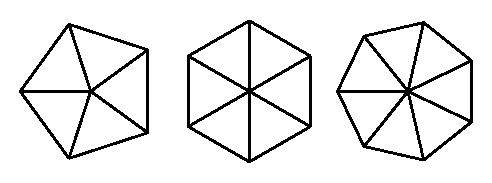
\includegraphics[height=0.9in]{figs/pies.eps}}

你可以从这里下载一个解决方案 \url{thinkpython.com/code/pie.py}。

\end{ex}

\begin{ex}
\index{字母}
\index{乌龟打字机}
\index{打字机,乌龟}

字母可以由一些基本元素组成,,如垂直或水平的线和曲线。使用最少的基本元素设计一种字体,并调用函数绘制字母。

你可以为每个字母写一个函数,命名为\verb"draw_a", \verb"draw_b"等,然后把你的函数放在 {\tt letters.py}的文件里。你可以从\url{thinkpython.com/code/typewriter.py}下载一个“乌龟打字机”来帮助你测试你的代码。

你可以从这里下载一个解决方案 \url{thinkpython.com/code/letters.py}。

\end{ex}


